\documentclass{article}
\usepackage[utf8]{inputenc}
\usepackage[a4paper, margin=1in]{geometry}

\title{Practica tmpfs}
\author{
    Karla Adriana Esquivel Guzman github.com/karlycaramelo \\
    Eric Giovanni Miguel Torres github.com/EricGiovanni \\
    María Ximena Lezama Hernández github.com/LezamaXi \\
    Gonzalo Vazquez Cruz github.com/truerandom \\
}
\date{Junio 2019}

\usepackage{natbib}
\usepackage{graphicx}

\begin{document}

\maketitle

\section{Introduccion}
EL objetivo de esta practica es crear una particion en ram para manejar datos del navegador en memoria principal de manera transparente.

\section{Desarrollo}
Se utilizo  tmpfs, rsync y cron para lo anterior.
Lo primero que si hizo fue localizar los datos del navegador.
\begin{figure}[h!]
\centering
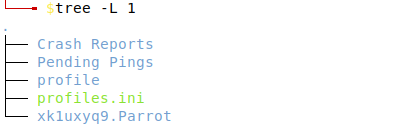
\includegraphics[scale=1]{imgs/estructura.png}
\caption{Estructura}
\label{fig:universe}
\end{figure}

Utilizaremos el perfil por default \\ 
\begin{figure}[h!]
\centering
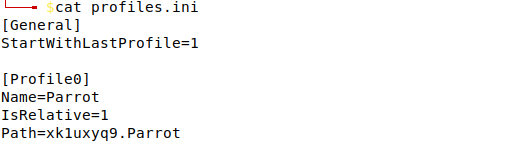
\includegraphics[scale=0.8]{imgs/profilesini.png}
\caption{Profiles ini}
\label{fig:universe}
\end{figure}
. \\ \\ \\ \\ \\ \\ \\ \\ \\ 

Montamos utilizando tmpfs agregando a /etc/fstab 
\begin{figure}[h!]
\centering
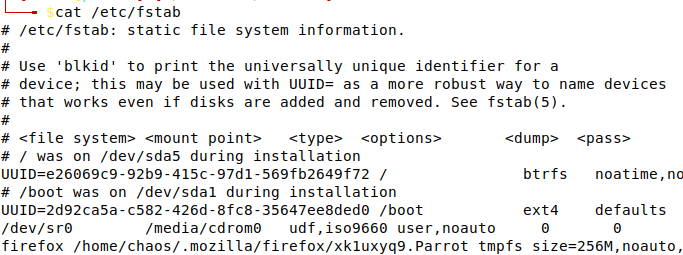
\includegraphics[scale=0.9]{imgs/fstab.png}
\caption{etc/fstab}
\label{fig:universe}
\end{figure}

. \\ \\ \\ 
Borramos y generamos el script para la sincronizacion
\begin{figure}[h!]
\centering
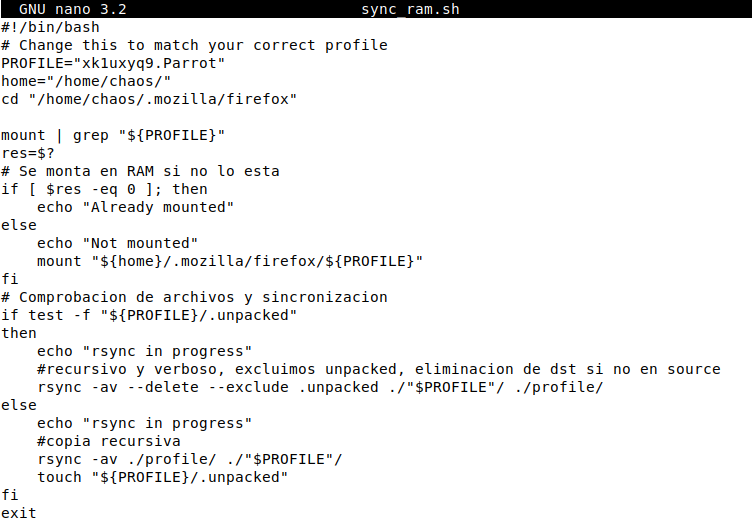
\includegraphics[scale=0.8]{imgs/script.png}
\caption{script}
\label{fig:universe}
\end{figure}
. \\ \\ \\ \\ \\ \\ 
Este script verifica si ya se encuentra en mount la carpeta de no ser asi lo monta.

\begin{figure}[h!]
\centering
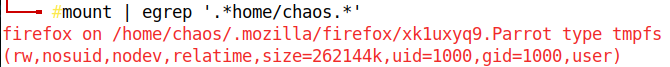
\includegraphics[scale=0.75]{imgs/perfil_en_ram.png}
\caption{Perfil en RAM}
\label{fig:universe}
\end{figure}
. \\ 
Si ya esta montada entonces hace la sincronizacion.
\begin{figure}[h!]
\centering
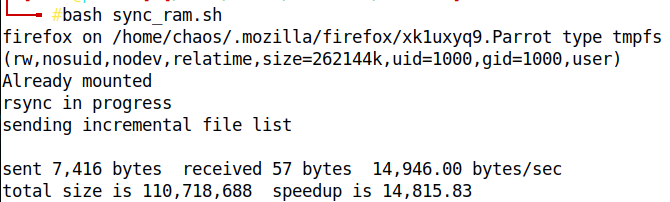
\includegraphics[scale=0.75]{imgs/sincronizando.png}
\caption{Sincronizacion utilizando el script}
\label{fig:universe}
\end{figure}
. \\
Ahora se verifica que puede abrirse firefox
\begin{figure}[h!]
\centering
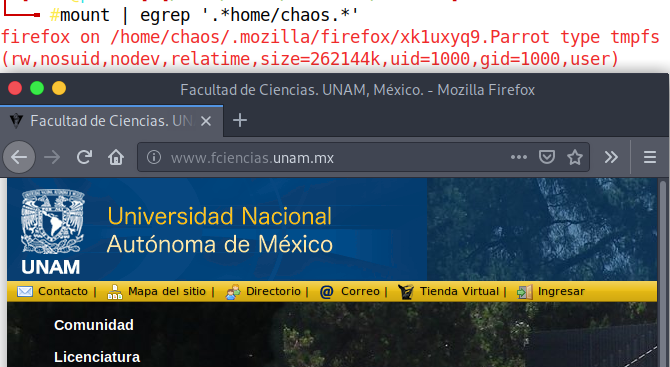
\includegraphics[scale=0.8]{imgs/firefox_corriendo.png}
\caption{firefox corriendo}
\label{fig:universe}
\end{figure}

Se define una tarea cron para sincronizar cada 5 minutos
\begin{figure}[h!]
\centering
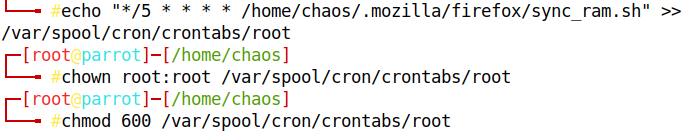
\includegraphics[scale=0.8]{imgs/crontab.png}
\caption{firefox corriendo}
\label{fig:universe}
\end{figure}

Por ultimo se define un script para ejecutar el navegador verificando que la particion se encuentre en ram.
\begin{figure}[h!]
\centering
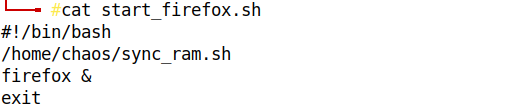
\includegraphics[scale=0.8]{imgs/start_firefox.png}
\caption{script startfirefox.sh}
\label{fig:universe}
\end{figure}

\section{Referencias}
http://www.webupd8.org/2013/02/keep-your-browser-profiles-in-tmpfs-ram.html \\
https://bbs.archlinux.org/viewtopic.php?id=131321 \\ 
https://soulchainer.github.io/posts/2014/12/20/exprimiendo-tmpfs/ \\
https://www.howtoforge.com/storing-files-directories-in-memory-with-tmpfs \\ 
https://www.verot.net/firefox\_tmpfs.htm \\
https://docs.oracle.com/cd/E19683-01/817-3814/6mjcp0r0l/index.html \\
https://github.com/eikevons/tmpfs-syncer
\end{document}
